\chapter{Project Activities and Outreach}
%%%%%%%%%%%%%%%%%%%%%%%%%%%%%%%%%%%%%%%%%%%%%%%%%%%%%%%%%%%%
%%%%%%%%%%%%%%%%%%%%  NEW SECTION   %%%%%%%%%%%%%%%%%%%%%%%%
%%%%%%%%%%%%%%%%%%%%%%%%%%%%%%%%%%%%%%%%%%%%%%%%%%%%%%%%%%%%
\setcounter{equation}{0}

%\nomenclature{ICAECT}{International Conference on Advances in Electrical, Computing, Communications and Sustainable Technologies}

\nomenclature{IEEE}{Institute of Electrical and Electronics Engineers}
\nomenclature{ICDICI}{International Conference on Data Intelligence and Cognitive Informatics}

\section{ICDICI-2024 Conference Submission}
The 5th International Conference on Data Intelligence and Cognitive Informatics (ICDCI 2024) invites global researchers, scholars, and industry professionals to explore the intersection of data intelligence and cognitive informatics. With a focus on understanding information processing systems, the conference aims to foster the development of advanced cognitive informatics technologies. The proof and reply email of the conference is shown in Figures \ref{fig:confSubmitted} and \ref{fig:confReply} respectively. 
\begin{itemize}

\item \textbf{Conference Name:} 5th International Conference on
Data Intelligence and Cognitive Informatics (ICDICI 2024)

\item \textbf{Publication:} Institute of Electrical and Electronics Engineers 
 (IEEE)

\item \textbf{Conference Dates:} 18\textsuperscript{th}-20\textsuperscript{th} November, 2024

\item \textbf{Date of Submission:} 2\textsuperscript{nd} May, 2024

\clearpage

\item \textbf{Acceptance Intimation:} 12\textsuperscript{th} September, 2024 

\item \textbf{Conference Website}: \textit{https://www.icdici.com/}

\item Notably this Conference was listed by the official conference searching site of the IEEE.

\item The selected paper immediately after the conference presentation will be submitted to IEEEXplore Digital Library.

\vspace{1cm}

\end{itemize}

\begin{figure}[h]
    \centering
    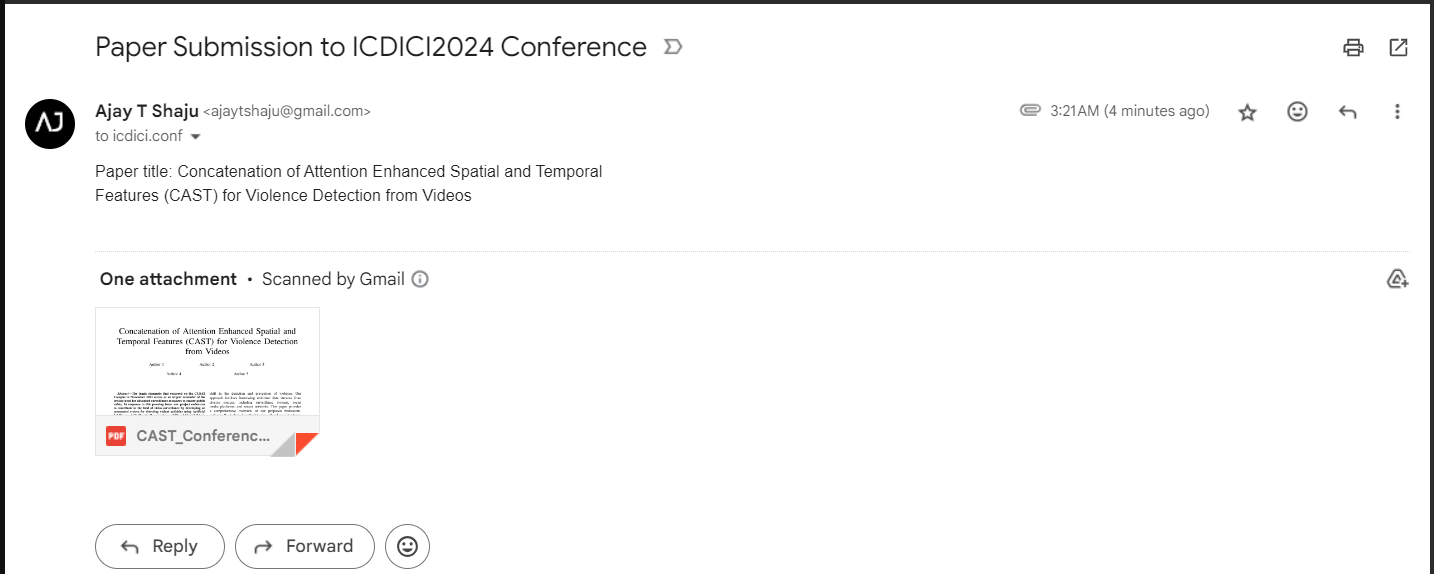
\includegraphics[width=0.8\linewidth]{Images/new_conf.png}
    \caption{Proof of Research Paper Submission to ICDICI2024 Conference}
    \label{fig:confSubmitted}
\end{figure}

\vspace{1cm}

\begin{figure}[h]
    \centering
    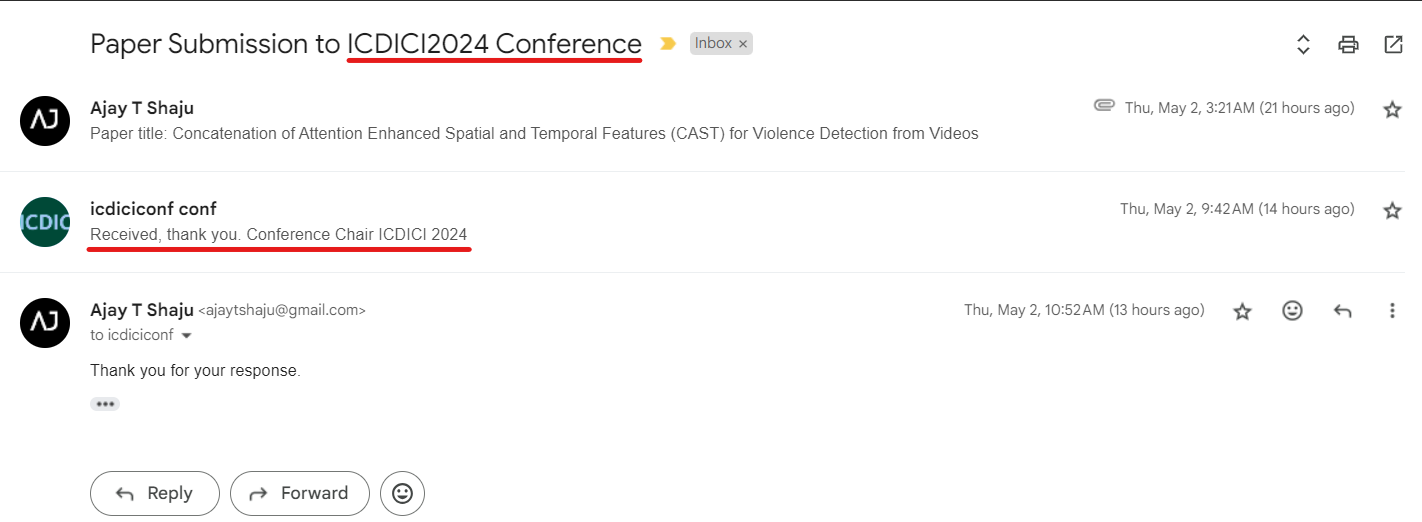
\includegraphics[width=0.8\linewidth]{Images/conf_reply.png}
    \caption{Reply - 'Paper Received' from ICDICI2024 Conference}
    \label{fig:confReply}
\end{figure}

\clearpage

\section{Carmel College Project Competition}

\begin{figure}[htbp!]
    \centering
    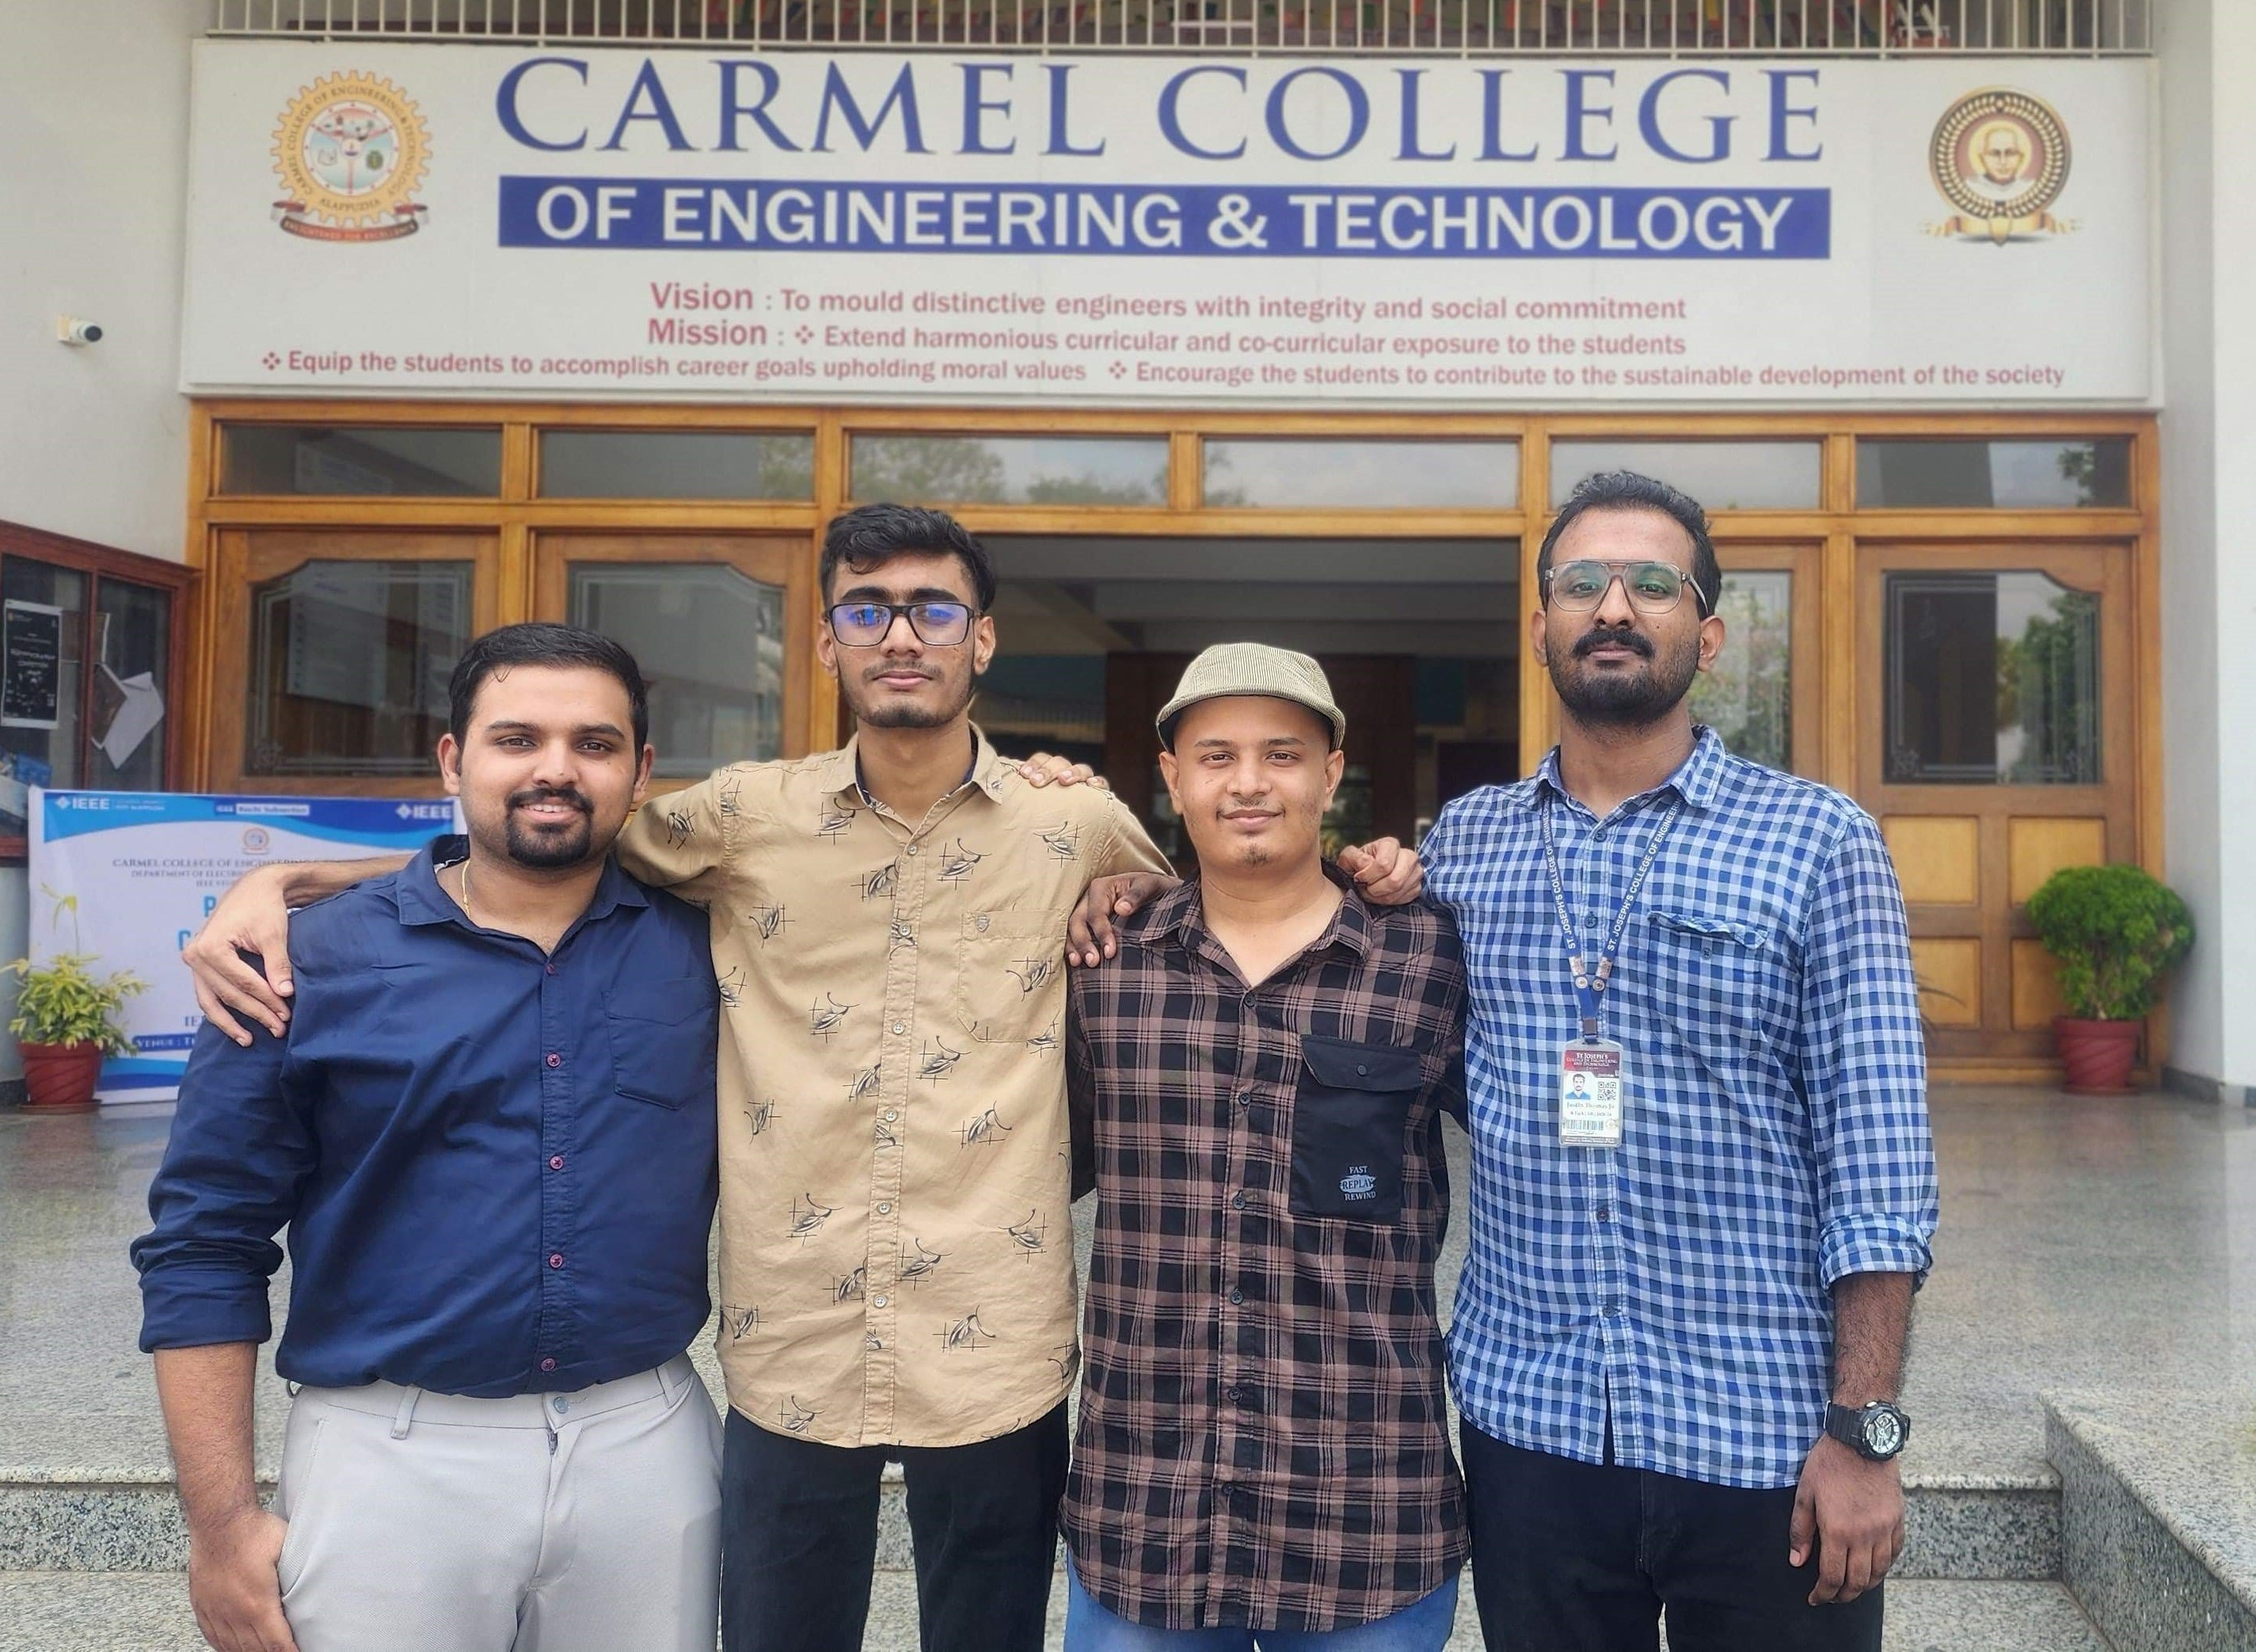
\includegraphics[width=0.85\linewidth]{Images/main_p_team_at_carmel_clg.jpg}
    \caption[Project Team members attending Project Competition]{Project Team Members Attending Project Competition at Carmel College of Engineering, Alappuzha held on 29\textsuperscript{th} April 2024. From left: Ajay T Shaju, Emil Saj Abraham, Vishnuprasad KG, and Justin Thomas Jo}
    \label{ccetComp}
\end{figure}

\vspace{1cm}

\noindent The team members participated in a project competition hosted at Carmel College of Engineering, Alappuzha Figure \ref{ccetComp}. The project presentation emphasized key features including the lightweight model, its scope, and notably the stampede incident at CUSAT served as the project's motivation, which seems to be easily understood by the judges of what the team has done. This experience provided an opportunity for all team members to showcase and exchange ideas with like-minded individuals, receiving valuable insights in return. Moreover, it enabled the team members to appreciate and learn from other projects presented at the competition.\\

% Further discussion about the details presented in Figure 6.1 can provide more insights.
%\ref{ccetComp}

% \begin{figure}[htbp!]
%     \centering
%     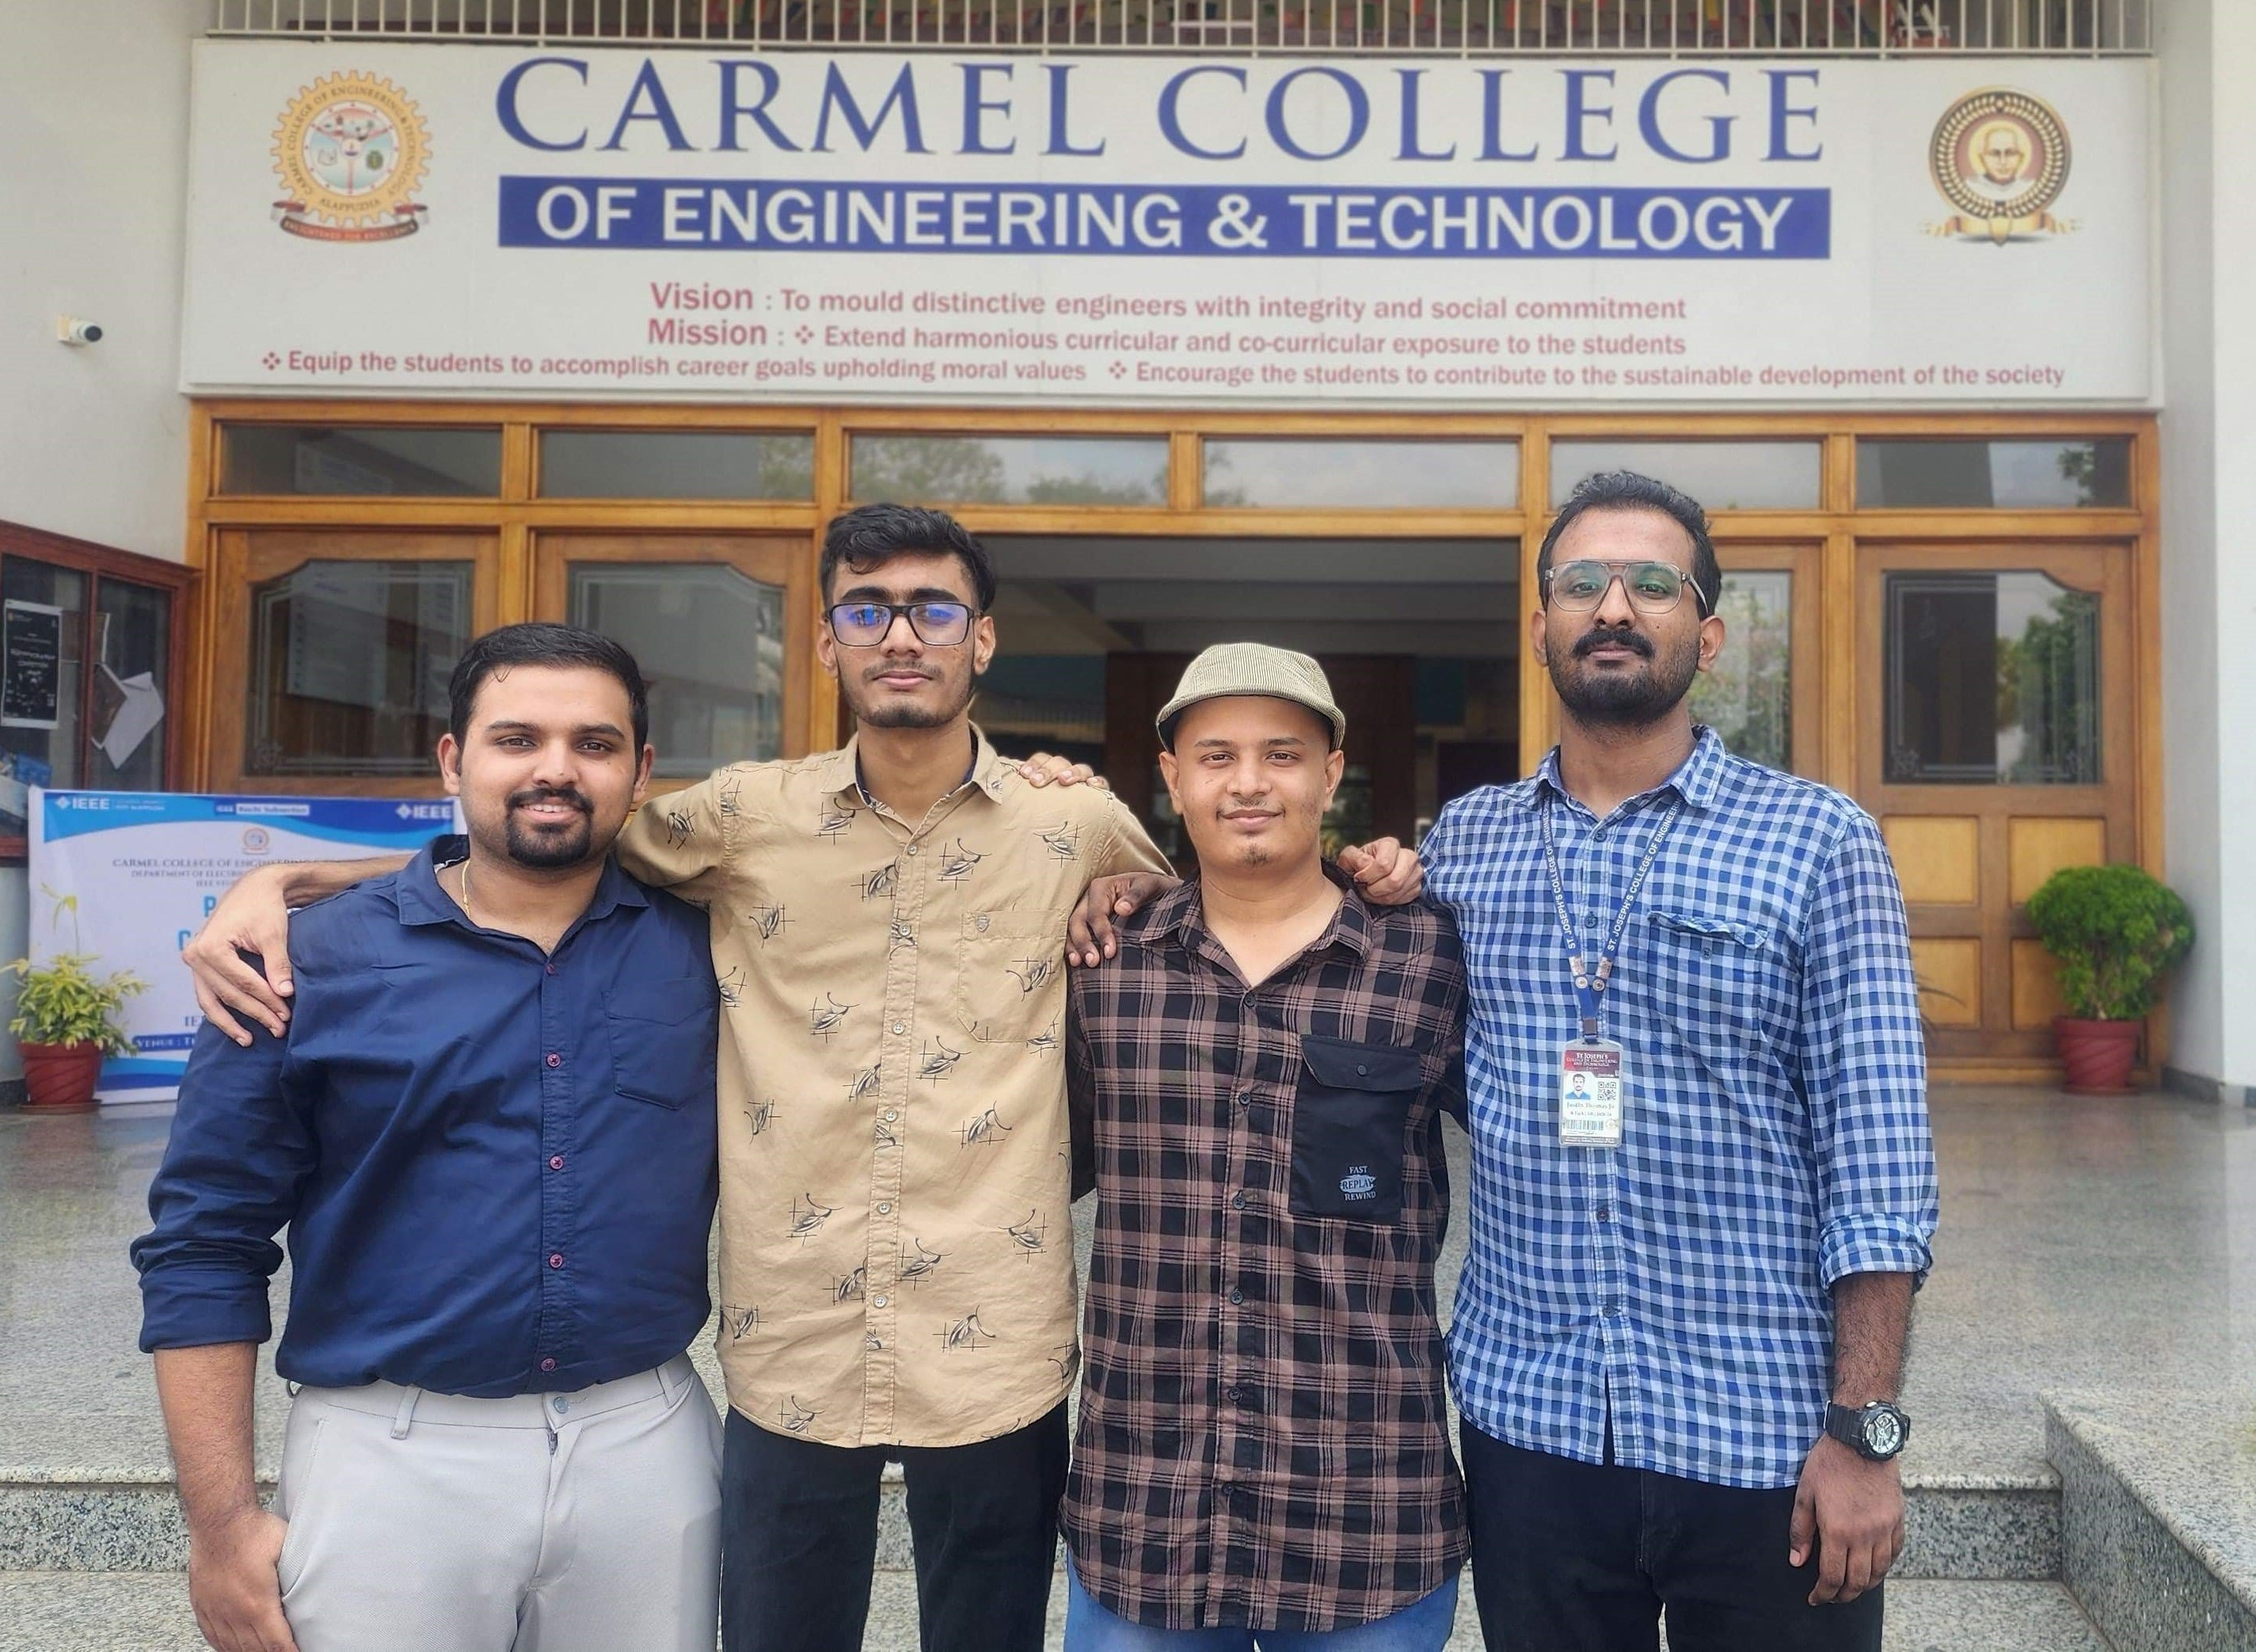
\includegraphics[width=0.7\linewidth]{Images/main_p_team_at_carmel_clg.jpg}
%     \caption[Project Team members attending Project Competition]{Project Team Members Attending Project Competition at Carmel College of Engineering, Alappuzha held on 29\textsuperscript{th} April 2024}
%     \label{ccetComp}
% \end{figure}

% \section{Indian Institute of Information Technology Kottayam}

% Participated in a workshop at IIIT-Kottayam, collaborating with professors who provided invaluable input for our violence mitigation project. Their keen interest in our concept led to enlightening exchanges of ideas and suggestions, enriching our understanding and fueling our project's development.

\lfoot{\textit{Departmant of Artificial Intelligence and Data Science, SJCET Palai}}
\renewcommand{\footrulewidth}{0.4pt}